\documentclass[11pt,a4paper]{article}
\usepackage[spanish,es-nodecimaldot]{babel}	% Utilizar español
\usepackage[utf8]{inputenc}					% Caracteres UTF-8
\usepackage{graphicx}						% Imagenes
\usepackage[hidelinks]{hyperref}			% Poner enlaces sin marcarlos en rojo
\usepackage{fancyhdr}						% Modificar encabezados y pies de pagina
\usepackage{float}							% Insertar figuras
\usepackage[textwidth=390pt]{geometry}		% Anchura de la pagina
\usepackage[nottoc]{tocbibind}				% Referencias (no incluir num pagina indice en Indice)
\usepackage{enumitem}						% Permitir enumerate con distintos simbolos
\usepackage[T1]{fontenc}					% Usar textsc en sections
\usepackage{amsmath}						% Símbolos matemáticos
\usepackage{listings}
\usepackage{color}

 
\definecolor{codegreen}{rgb}{0,0.6,0}
\definecolor{codegray}{rgb}{0.5,0.5,0.5}
\definecolor{codepurple}{rgb}{0.58,0,0.82}
\definecolor{backcolour}{rgb}{0.99,0.99,0.99}
 
\lstdefinestyle{mystyle}{
    backgroundcolor=\color{backcolour},   
    commentstyle=\color{codegreen},
    keywordstyle=\color{magenta},
    numberstyle=\tiny\color{codegray},
    stringstyle=\color{codepurple},
    basicstyle=\footnotesize,
    breakatwhitespace=false,         
    breaklines=true,                 
    captionpos=b,                    
    keepspaces=true,                 
    numbers=left,                    
    numbersep=5pt,                  
    showspaces=false,                
    showstringspaces=false,
    showtabs=false,                  
    tabsize=2
}
 
\lstset{style=mystyle, language=Python}

% Comando para poner el nombre de la asignatura
\newcommand{\asignatura}{Programación Lúdica}
\newcommand{\autor}{José María Sánchez Guerrero}
\newcommand{\titulo}{Propuesta}

% Configuracion de encabezados y pies de pagina
\pagestyle{fancy}
\lhead{José María Sánchez Guerrero, Antonio Godoy González}
\rhead{\asignatura{}}
\lfoot{Grado en Ingeniería Informática}
\cfoot{}
\rfoot{\thepage}
\renewcommand{\headrulewidth}{0.4pt}		% Linea cabeza de pagina
\renewcommand{\footrulewidth}{0.4pt}		% Linea pie de pagina

\begin{document}
\pagenumbering{gobble}

% Pagina de titulo
\begin{titlepage}

\begin{minipage}{\textwidth}

\centering


\includegraphics[scale=0.5]{img/ugr.png}\\

\textsc{\Large \asignatura{}\\[0.2cm]}
\textsc{GRADO EN INGENIERÍA INFORMÁTICA}\\[1cm]

\noindent\rule[-1ex]{\textwidth}{1pt}\\[1.5ex]
\textsc{{\Huge \titulo\\[0.5ex]}}
\noindent\rule[-1ex]{\textwidth}{2pt}\\[3.5ex]

\end{minipage}

\vspace{0.5cm}

\begin{minipage}{\textwidth}

\centering

\textbf{Autores}\\ {\autor{}}\\{Antonio Godoy González}\\[2ex]
\textbf{Rama}\\ {Computación y Sistemas Inteligentes}\\[2.5ex]
\vspace{0.3cm}


\includegraphics[scale=0.3]{img/etsiit.jpeg}

\vspace{0.7cm}
\textsc{Escuela Técnica Superior de Ingenierías Informática y de Telecomunicación}\\
\vspace{1cm}
\textsc{Curso 2019-2020}
\end{minipage}
\end{titlepage}

\pagenumbering{arabic}
\thispagestyle{empty}				% No usar estilo en la pagina de indice

\newpage

\setlength{\parskip}{1em}


\section*{Introducción}

Presentamos el videojuego llamado provisionalmente ''\textit{Black Lights}'' realizado gracias al motor
de código abierto Godot Engine. Los integrantes del proyecto somos José María Sánchez Guerrero y Antonio
Godoy González.

\section*{Descripción del videojuego}

''\textit{Black Lights}'' es un juego de acción en 2D, siguiendo un estilo artístico \textit{pixelart} y
ubicado en un mundo futurista. Vamos a manejar a un personaje cuya historia (aún por detallar) le lleva
a superar distintos desafíos, ya sean enfrentarse a enemigos, resolver puzzles o tomar importantes
decisiones.

Como hemos mencionado, el género del juego es de acción. Va a ser un juego en 2D \textit{pixelart} con
movimiento tipo \textit{Top-down}, donde incorporamos un \textit{dash} para simular el salto. El mapa
estará dividido por habitaciones o escenas que irán a medida de cómo se suceda la historia.

El público al que va dirigido será a cualquier persona mayor de los 12 años, ya que puede ser un poco
sangriento o la historia puede ser dura. Pese a poder jugar multijugador, es un juego con historia, por
lo que no está hecho para jugar partidas rápidas como puede ser \textit{League of Legends} o \textit{Counter
Strike}. Está hecho para los amantes de las buenas historias y los que esperan una segunda parte nada más
terminar la primera.

\section*{Estudio de mercado}

Los juegos similares o del mismo género son:
\begin{itemize}
    \item \textbf{Hollow Knight - Team Cherry}. Pese a ser un juego 2D con scroll lateral, en vez de \textit{Top-down}
    como el nuestro, la jugabilidad que deseams obtener es la misma, con un movimiento similar pero en
    las 4 direcciones, y con un sistema de logros, objetivos e historia muy parecidos. Lo que nos va a
    diferenciar de este (aparte del tipo de 2D) es el modo cooperativo que nosotros sí implementaremos.
    \begin{figure}[H]
        \centering
        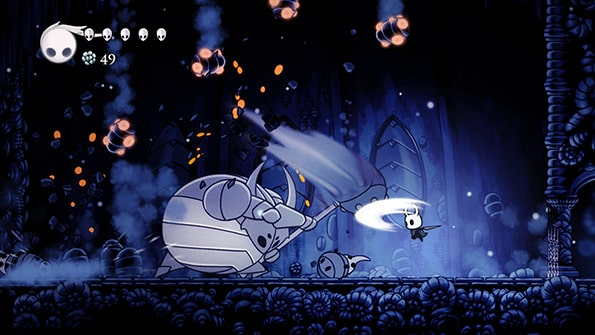
\includegraphics[scale=0.6]{img/hollow.jpg}
        \caption{https://hollowknight.com/}
    \end{figure}

    \item \textbf{HyperLight Drifter - Heart Machine}. Es el juego más similar al nuestro, tanto en
    estilo, arte o jugabilidad. No obstante, al igual que el anterior, este juego está hecho sólo para
    un jugador.
    \begin{figure}[H]
        \centering
        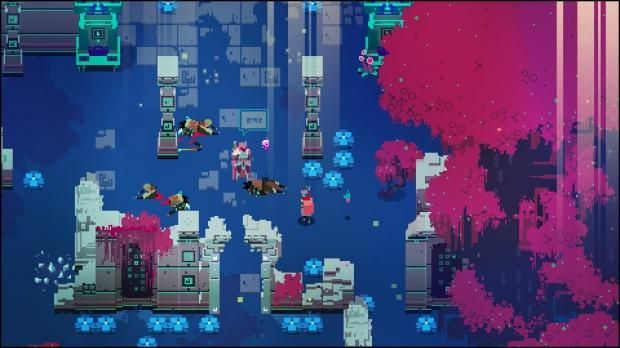
\includegraphics[scale=0.6]{img/drifter.jpg}
        \caption{https://heartmachine.com/}
    \end{figure}

    \newpage
    \item \textbf{Moonlighter - Digital Sun}. También muy similar al anterior, pero con un arte un poco más
    simple (que será el que realizaremos en nuestro juego). Este juego tampoco tiene cooperativo y el modo de
    juego está más dirigido al farmeo completando \textit{rooms} para ello, en vez de contar una historia.
    \begin{figure}[H]
        \centering
        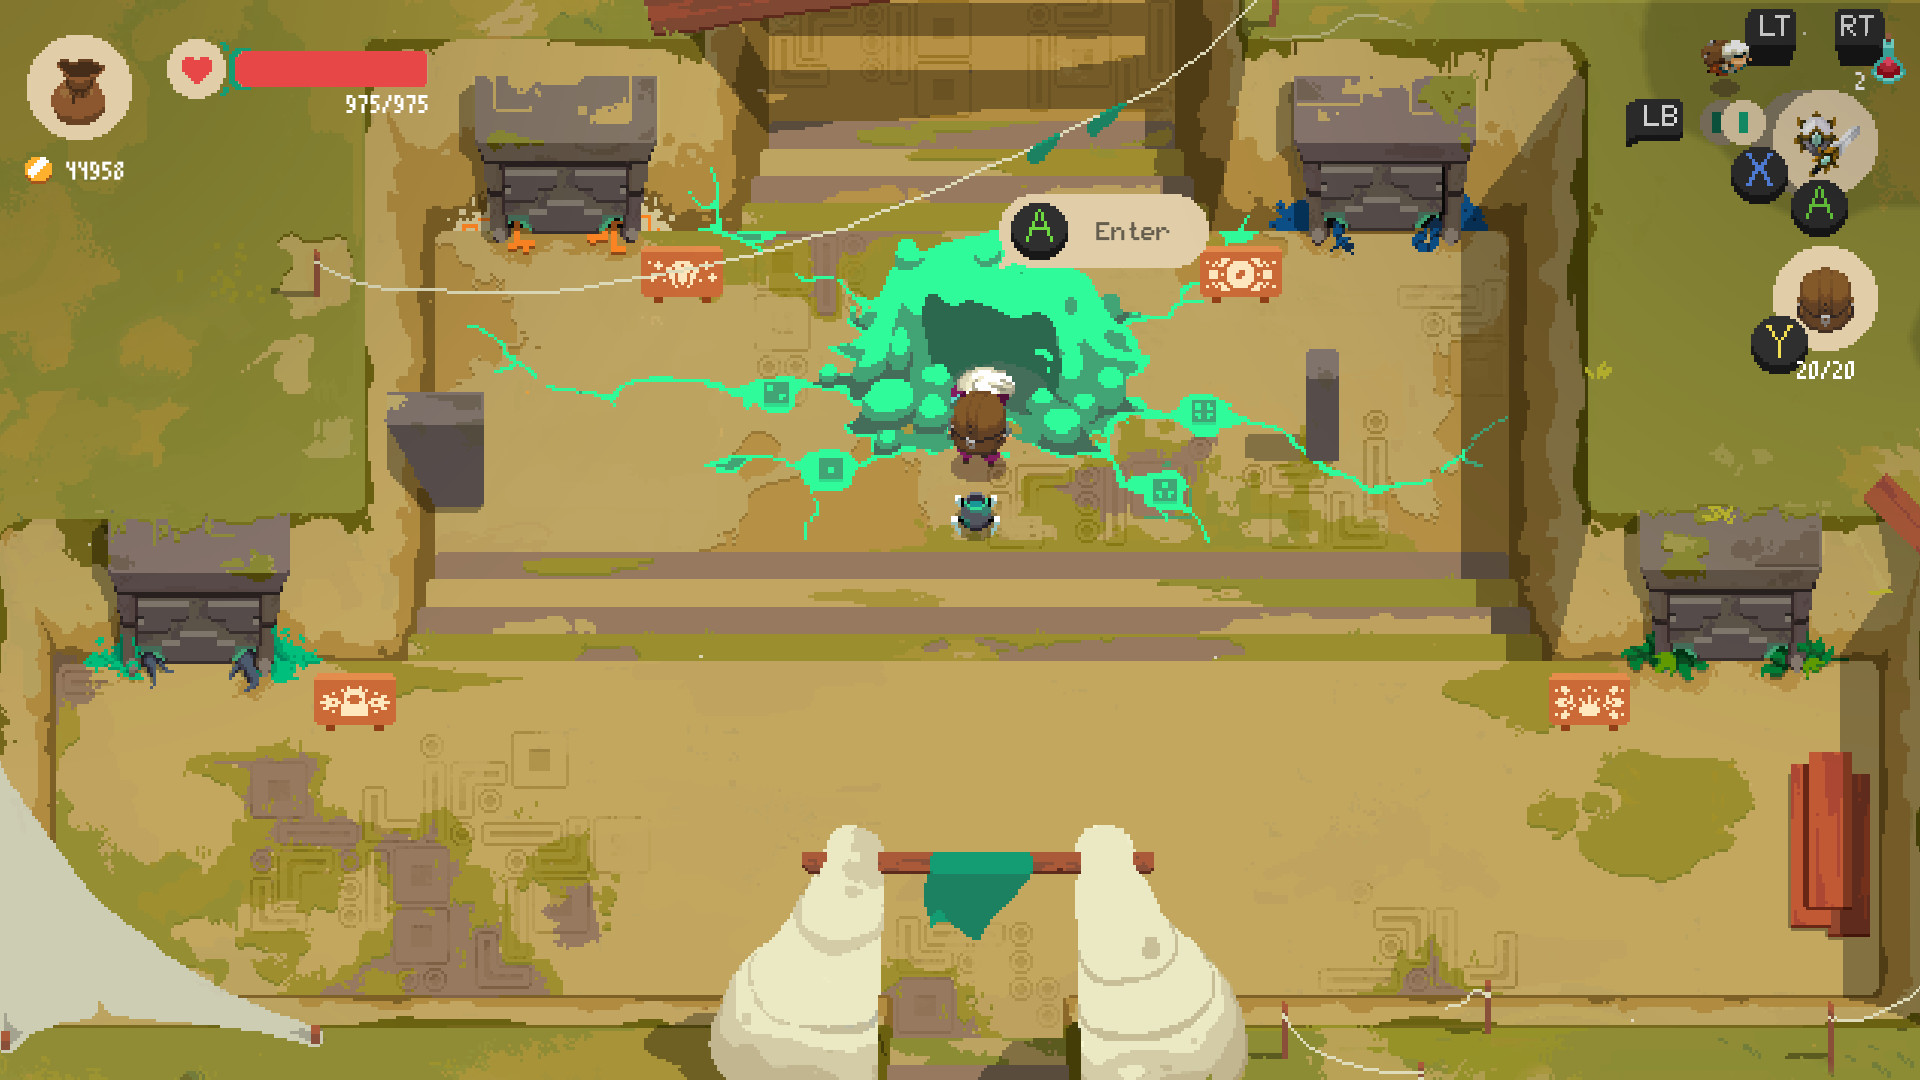
\includegraphics[scale=0.19]{img/moon.jpg}
        \caption{https://heartmachine.com/}
    \end{figure}

\end{itemize}



\end{document}